\subsection{Historia: ¿Cómo llegamos a donde estamos?}
\label{nube:historia}

Como desarrolladores y analistas del \cespi, dependencia de la \unlp encargada de fomentar, implementar y administrar TICs, hemos participado del relevamiento, la implementación, la puesta en producción y el mantenimiento de varias aplicaciones web de uso diario por los agentes de las distintas Unidades Académicas y demás Dependencias administrativas de esta Alta Casa de estudios. Así, en el transcurso de más de 7 años de experiencia, hemos migrado entre distintos paradigmas arquitectónicos en el desarrollo de las aplicaciones y su intercomunicación.

En este capítulo haremos una reseña de lo ocurrido en este tiempo, separando en etapas marcadas por los distintos enfoques que fuimos dando a la problemática de alimentar las distintas aplicaciones que desarrollamos para la UNLP, indicando las razones y decisiones que tomamos en cada ocasión, y que dan origen a este análisis que será la base para la futura etapa de implementación de la nube de servicios integrados.


\subsubsection{Prefacio: ¿Qué es la nube de servicios de la UNLP?}
\label{nube:prefacio}

Liminarmente creemos conveniente y necesario explicar \textit{qué} es la nube de la que hablaremos en este trabajo. Por simplicidad, y para no develar detalles técnicos que aún no queremos mencionar, nos centraremos en los aspectos funcionales, en el \textit{qué} y no en el \textit{cómo}, de la fuente de información unificada que utilizamos en las aplicaciones que desarrollamos a diario para la \unlp.

La nube de servicios es un solo sistema web que concentra la información que permite a distintas aplicaciones web, desarrolladas en la \direccionDesarrollo para uso interno de la UNLP, unificar datos y a partir de esta unificación combinar y correlacionar la información que cada una posee. Contiene y provee datos que van desde identificadores únicos para diferentes tipos de documento (como ser \textit{“1 equivale a Documento Nacional de Identidad”}, \textit{“2 a Libreta de Enrolamiento”}, o \textit{“5 a Pasaporte”}, por poner algunos ejemplos), pasando por valores concretos para identificar las Unidades Académicas o Dependencias de la Universidad (\textit{“33 para la Facultad de Informática”}, \textit{“26 para el CeSPI”}, etcétera), hasta datos concretos de las personas relacionadas a la UNLP (\textit{“000000000000000000000031988189 es \nahuelcuesta, alumno de la \facultad, docente con dos cargos de dedicación simple en la misma Unidad Académica”}, o \textit{“000000000000000000000027855859 es \miguelcarbone, alumno de la \facultad, docente con un cargo de dedicación simple en esa UA”}, por tomar dos casos). Mediante los servicios que brinda esta nube se pueden consultar, sin posibilidades de realizar operaciones modificatorias o destructivas, los siguientes grupos de datos:

\begin{itemize}
  \item Datos de referencia:
  \begin{itemize}
    \item Tipos de documento
    \item Géneros
    \item Estados civiles
    \item Países, provincias, partidos y localidades
    \item Unidades Académicas de la UNLP
  \end{itemize}
  \item Información académica:
  \begin{itemize}
    \item Carreras
    \item Planes de estudios
    \item Materias
    \item Títulos otorgados
  \end{itemize}
  \item Sobre las personas vinculadas a la UNLP (Alumnos y Personal):
  \begin{itemize}
    \item Datos personales
    \item Datos de contacto
  \end{itemize}
  \item Sobre los cargos del personal de la UNLP (Docentes, Nodocentes y Autoridades Superiores):
  \begin{itemize}
    \item Información histórica
    \item Quién ocupa el cargo
    \item A qué Unidad Académica pertenece
    \item En qué situación se encuentra
    \item Los recibos de sueldo del cargo
  \end{itemize}
\end{itemize}

Las aplicaciones que consumen esta información, los \textit{clientes de la nube}, acceden mediante distintos servicios web a los datos que desean. Por ejemplo, un servicio provee todos los tipos de documento que la nube conoce, incluyendo el identificador único de cada tipo de documento y su descripción; mientras que otro servicio provee la información de contacto detallada de un empleado de la UNLP. De esta forma los clientes deben conocer qué servicios brinda la nube y cómo acceder a cada uno de ellos para poder acceder a la información.

Dada la cantidad de aplicaciones que hoy día utilizan los servicios de esta nube para su funcionamiento básico, es de suma importancia -para las tareas que desempeña nuestra Dirección- que su funcionamiento y \eng{performance} sean óptimos, que la dificultad para mantenerla sea mínima y que la tolerancia a fallos o resiliencia de los servicios sea adecuada.

Habiendo hecho esta breve descripción de qué es la nube de servicios, hemos brindado el contexto necesario para comenzar a explicar su evolución, ahora sí incluyendo detalles técnicos sobre su implementación.


\subsubsection{El génesis: aplicaciones como islas}
\label{nube:etapa0}

En un principio, cada aplicación funcionaba como un sistema autónomo en su totalidad: no existía comunicación entre los sistemas que estábamos implementando, que hasta ese momento eran relativamente pocos. Cada una definía sus propios datos, tanto los de su dominio particular como aquellos más generales - entiéndase por estos últimos información que categoriza los datos de dominio ya sea georeferenciando las ubicaciones, a las personas por género, por su Dependencia de trabajo o estudio, los documentos de identidad por su tipo, etcétera -. Si bien a simple vista esto puede presentar un claro punto de \eng{refactor} para evitar un inminente problema de duplicación y desnormalización de los datos, en ese punto de madurez de los requerimientos que llegaban a nuestra oficina la necesidad no era evidente y mucho menos imprescindible.

El problema no se hizo esperar, al poco tiempo, fue creciendo la necesidad de comunicar las aplicaciones por diferentes razones que se desprendían de los inconvenientes que comenzaban a surgir con el diseño planteado para las aplicaciones:

\begin{itemize}
  \item \textbf{Normalización de datos:} las distintas aplicaciones manejaban los datos generales (o de referencia, como los llamaremos de aquí en más) de diferentes maneras, con distintas convenciones, y - lo que es aún más problemático - con diferentes valores concretos para indicar los mismos datos. Por ejemplo, en una aplicación el género femenino era representado con un valor entero 1, mientras que en otra ése era el valor asignado al género masculino. Otro ejemplo más complejo eran las Dependencias de la Universidad, que en cada aplicación tenían diferentes identificadores y descripciones. Esta falta de normalización en los datos hacía virtualmente imposible cruzar la información entre distintas aplicaciones y hacía más compleja cualquier actualización necesaria a esos datos de referencia.\\
  A esto se le suma el mantenimiento de los datos, es decir, siguiendo con el ejemplo de las Dependencias, si era necesario incorporar una nueva, la misma debía ser cargada en cada una de las aplicaciones que utilizaban ese dato de referencia.

  \item \textbf{Unificación de la forma de obtener la información:} este esquema disconexo también acarreaba otro problema oculto en su organización que era la falta de una interfaz unificada de acceso a los datos de referencia. Así como cada aplicación definía sus datos, esto también implicaba definir el acceso a los mismos, lo cual acababa en tantos métodos distintos de acceso a los datos de referencia como aplicaciones se tenían. Si bien se intentaba mantener un criterio uniforme, las más pequeñas mejoras o personalizaciones en la forma de acceso a un dato de referencia realizadas en una aplicación hacían que ésta fuera diferente del resto. Por ejemplo, en algunas aplicaciones se implementaban mecanismos opcionales de \eng{caching} para agilizar algunas consultas repetitivas a los datos de referencia, requiriendo de un parámetro específico para indicar si se deseaba o no utilizar esa \eng{cache}; mientras que en otras aplicaciones esta noción no existía, y en su lugar implementaban agregaciones de los datos de referencia diferentes al resto porque la aplicación los necesitaba. Este era claramente un escenario poco deseable, principalmente por la característica de nuestro equipo de trabajo: éramos un grupo de desarrolladores relativamente pequeño en el que todos participábamos de la implementación de todas las aplicaciones, por lo que el pivoteo de una aplicación a la otra tenía un \eng{overhead} innecesario a la hora de analizar qué intentaba realizar la misma operación de obtención de datos en una u otra implementación.

  \item \textbf{Eliminar la repetición de datos y de código:} como se esbozó en los puntos anteriores, la falta de estandarización y uniformidad de la información se vio reflejada en las diferentes implementaciones de unidades funcionalmente similares (por no decir idénticas). Esto hizo que los diferentes proyectos de las aplicaciones tuvieran diversas implementaciones (a nivel de código) para realizar las mismas tareas, y que los datos de referencia que éstas manejaban se repitieran (aunque con las diferencias antes mencionadas) en cada una.
\end{itemize}


\subsubsection{Primera iteración: eliminando la repetición y normalizando los datos}
\label{nube:etapa1}

Ante la creciente cantidad de aplicaciones, los problemas antes enumerados se hacían cada vez más evidentes. Fue entonces que se decidió pasar a un nuevo enfoque sobre el problema: unificar los datos y el código utilizados en las distintas aplicaciones mediante la implementación de clases y objetos reutilizables en ellas.

Este tipo de solución fue relativamente fácil de implementar dada la homogeneidad de frameworks y librerías que nuestras aplicaciones poseían de base. En ese entonces nuestro \eng{stack} de desarrollo estaba principalmente conformado por PHP 5.3, el \eng{framework} \gls{fw:symfony} y bases de datos MySQL, lo cual nos permitió escribir una única vez una librería (o \eng{plugin}, en la terminología del \eng{framework} utilizado) e incluirla en todos los proyectos muy fácilmente. Al centralizar los datos y la lógica de acceso a los mismos en estas clases reutilizables, eliminábamos la repetición de código y datos, y normalizábamos los datos comunes que las aplicaciones utilizaban; y al mismo tiempo simplificábamos el mantenimiento de estas aplicaciones ya que cualquier cambio o solución a un error detectado en las clases de referencia se efectuaba en un único lugar (el \eng{plugin} que las contenía) y se replicaba en las aplicaciones con sólo actualizar la versión del \eng{plugin} disponible en cada aplicación desde nuestro sistema de control de versiones de código\footnote{\gls{scm:subversion} y \gls{scm:git} son las dos herramientas para versionar el código de los proyectos que hemos utilizado. El pasaje de \gls{scm:subversion} a \gls{scm:git} fue por los beneficios que este último ofrecía en comparación al primero, principalmente el sistema de ramas (\eng{branching}) que utiliza, su esquema descentralizado y el sustancialmente menor tamaño final de los repositorios de código.}.

Las clases de referencia consistían en una interfaz común de acceso a la información que éstas contenían y los datos propiamente dichos escritos en el código. A modo ilustrativo, presentamos aquí un extracto de la clase que contenía los tipos de documento, y un ejemplo de uso de la misma:

%%%
%%% TODO: Insertar acá contenido de https://gist.github.com/ncuesta/51abb9c3ca3420249052
%%%

Si bien en principio este acercamiento al problema es altamente beneficioso en comparación a la situación que intenta mejorar, está claramente lejos de ser una solución óptima. En cierto modo, este nuevo enfoque fue el pilar fundamental para la evolución hacia soluciones mejores y más complejas.

El inconveniente con este enfoque era que pese a eliminar la repetición que existía y normalizar los datos, introducía nuevos problemas:

\begin{itemize}
  \item Si bien los datos de referencia ahora se encontraban unificados a lo largo de todas nuestras aplicaciones, éstos se encontraban \textit{embebidos} estáticamente en el código\footnote{En términos más técnicos, nos encontrábamos ante un indeseable caso de \eng{hard-coded data}. Estábamos unificando nuestra lógica de negocios (código) con los datos del dominio, todo escrito en el fuente de nuestra librería.}. Cada cambio en la información implicaba lanzar una nueva versión del \eng{plugin} para poder reflejarlo en las aplicaciones.

  \item Cada actualización en la lógica de obtención de los datos (o en los datos mismos, por lo detallado en el punto anterior) implicaba actualizar todas las aplicaciones que hacían uso de la librería. Este acoplamiento entre las aplicaciones y la fuente de datos de referencia era otro grave problema que tenía esta organización, ya que todas las aplicaciones seguían incluyendo los datos dentro de sí.
\end{itemize}


\subsubsection{Segunda iteración: haciendo dinámicas las fuentes de datos}
\label{nube:etapa2}

Luego de la primera iteración en que logramos unificar los datos de referencia, y una vez pasado el periodo inicial de estabilización de la nueva solución, comenzamos a planificar la siguiente mejora a la forma en que disponíamos de la información: hacer dinámicas las fuentes de datos de referencia.

Si bien el nuevo \eng{approach} hasta este momento subsanaba los inconvenientes que conllevan la repetición y falta de normalización en los datos, éste traía acarreada  la poco deseable nueva situación de que los datos de referencia de nuestras aplicaciones eran estáticos y se encontraban escritos directamente en el código. Como se detalló en la sección anterior, esto dificultaba la actualización de cualquier dato en nuestras aplicaciones y  acoplaba el código con los datos, lo cual es considerado un \gls{term:antipatron}. Entonces el paso lógico era llevar esos datos a una fuente dinámica, como una base de datos, administrable desde alguna interfaz amigable, a la que las aplicaciones tuvieran acceso y pudieran consultar.

Fue así que una vez más la homogeneidad de nuestros desarrollos nos facilitó la tarea: modificamos nuestro \eng{plugin} de \gls{fw:symfony} existente para que las clases que antes contenían los datos directamente embebidos dentro de ellas, ahora fuesen abstracciones de tablas en una base de datos dedicada a los datos de referencia. Con este -relativamente sencillo- cambio en nuestro código, la librería común ya soportaba un \gls{term:backend} dinámico para las fuentes de datos y por ende nuestras aplicaciones daban un salto de calidad al utilizar estos nuevos datos de referencia administrables sin tocar código.

Así, pese los beneficios obtenidos, apareció un nuevo problema: para poder brindar soporte a esta nueva solución debíamos, para cada aplicación que los utilizace, incluir los datos de conexión a la base de datos de referencia y permitir en nuestra infraestructura que la aplicación tenga acceso a esa base de datos central\footnote{Esto implicaba habilitar reglas en firewalls y agregar privilegios a usuarios de la base de datos para conectarse desde distintos hosts.}. Además de estos nuevos requerimientos para cada aplicación, se acarreaban nuevos potenciales inconvenientes:

\begin{itemize}
  \item Si bien nuestras aplicaciones sólo consultaban la información de referencia que esta base de datos contenía, en caso que los privilegios de acceso a la base de datos fueran demasiado permisivos, se corría el riesgo que cualquier sistema pudiera (accidentalmente o mediante un ataque malintencionado) modificar o borrar la información común a todas las aplicaciones.

  \item Esta nueva arquitectura ponía a ese nodo central de la base de datos bajo gran stress en momentos que el uso de las aplicaciones se incrementaba, por lo que se debía implementar un mecanismo de \eng{caching} artesanal, local a cada aplicación, que aliviase esa carga. Esta técnica, si bien mitigaba el problema, estaba lejos de ser una solución al mismo, ya que cada aplicación consultaría por separado el mismo conjunto de datos al menos una vez cada cierto período de tiempo, lo almacenaría en su caché local, y manejaría de forma desconexa el tiempo que esos datos se consideraban \textit{frescos}, independientemente del resto de las aplicaciones.
\end{itemize}

El beneficio obtenido al dinamizar la fuente de nuestros datos de referencia, quitando los datos concretos del código del \eng{plugin} de acceso a los mismos, y simplificando la actualización de esta información de forma independiente a nuestras aplicaciones, fue enorme. Pero esta solución aún no eliminaba por completo el acoplamiento entre nuestras aplicaciones y la fuente de datos de referencia. De hecho, introducía nuevos niveles de acoplamiento al hacer que nuestras aplicaciones deban tener acceso a una base de datos (común) y mantener la información de acceso a ésta; al hacer que las distintas aplicaciones puedan potencialmente modificar esa información común sin que ésto sea deseable; al requerir que las políticas de infraestructura permitan la comunicación directa desde múltiples aplicaciones al nodo de la base de datos; al necesitar agregar privilegios de acceso a la base de datos de referencia; y al obligar a las aplicaciones a conocer la implementación interna de cada tipo de dato (su estructura en la base de datos) para poder accederla directamente.


\subsubsection{Tercera iteración: unificando el acceso a la información y desacoplando las componentes}
\label{nube:etapa3}

En este punto, la cantidad de aplicaciones conectadas a la nube de servicios que habíamos desarrollado había alcanzado prácticamente la decena. Este creciente número de sistemas que debían acceder directamente a las fuentes compartidas de información hacía evidente la necesidad de un nuevo \gls{term:refactor}: cada aplicación necesitaba ser mantenida no sólo por su dominio propio sino también ante cualquier modificación realizada a las fuentes de información de referencia, además debíamos tener el cuidado y la conducta de no realizar operaciones de escritura desde ninguna de las \gls{term:aplicacionessatelitales} de la nube sobre los datos que ésta última contiene.

Estas complicaciones adicionales a la implementación de los sistemas propiamente dichos nos dejaban en claro la premisa principal con la cual debíamos replantear el diseño de la nube: la información debía aislarse, asegurarse y ser de sólo lectura, pero sin hacer más complejo el acceso a la misma.

Con esa premisa como \eng{leitmotiv}, decidimos centralizar en un lugar los datos que las aplicaciones necesitaban consumir: una única fuente que serviría la información mediante una interfaz web a sus clientes. Con este cambio en el diseño estaríamos cumpliendo tres de los cuatro pilares que guiaban esta etapa del desarrollo:

\begin{itemize}
  \item La información se encontraría aislada ya que al tener una única aplicación accediéndola (el nuevo proveedor centralizado de información) dejaría de ser necesario que cada aplicación se conecte directamente a la base de datos que hasta ese momento era compartida.

  \item Al tratarse de una aplicación, asegurar la información sería cuestión de definir un protocolo de acceso a la misma con políticas concretas sobre quién y cómo podría consumirla.

  \item De manera similar al punto anterior, hacer que el acceso a la información fuera de sólo lectura sería cuestión de no proveer medios para que los clientes realicen escrituras sobre la misma.
\end{itemize}

Para el punto restante necesitábamos definir la interfaz y el protocolo mediante los cuales las \gls{term:aplicacionessatelitales} accederían a la información. Tratándose de aplicaciones web separadas en distintos servidores la forma evidente de implementar la comunicación sería utilizando la web como medio, pero restaba definir cómo dialogarían las aplicaciones cliente con el proveedor para obtener los datos. En nuestra experiencia hasta ese momento habíamos trabajado con \glspl{ws:webservice} para realizar comunicaciones entre diferentes aplicaciones mediante la web, pero a partir de esa experiencia teníamos nuestras reservas sobre este estándar, principalmente:

\begin{itemize}
  \item Su implementación nos resultaba excesivamente complicada, al involucrar muchos puntos de acción y acababa siendo propensa a errores humanos. El protocolo general de los \glspl{ws:webservice} contiene diversos elementos que intervienen en cada parte de la comunicación entre los dos sistemas:
  \begin{itemize}
    \item El proveedor del servicio utiliza \gls{ws:wsdl} para describir qué servicios brinda, de qué forma deben accederse, qué formato deben tener los parámetros, y cómo estará estructurada la respuesta. Esta definición de los servicios se mantenía en un documento \gls{lang:xml} que debía ser actualizado cada vez que los datos, puntos de acceso, parámetros esperados y/o la estructura del proyecto cambiaba, agregando un punto más de falla humana al proceso de desarrollo.

    \item El proveedor y el cliente se comunican utilizando el framework \gls{ws:soap} para intercambio de mensajes y codifican en documentos \gls{lang:xml} los mensajes que intercambiarán. Este protocolo de acceso a la información agrega un \eng{overhead} a la comunicación por sobre lo que cualquier comunicación web, basada en el protocolo \gls{proto:http}\footnote{En secciones siguientes desarrollaremos en mayor profundidad las partes principales de este protocolo que atañen al presente trabajo a fin de dar un marco tecnológico concreto a nuestras definiciones.}, que sabíamos podía ser evitado si utilizásemos otro mecanismo para estos fines.
  \end{itemize}

  \item Tal como indicamos en el punto anterior, este protocolo agrega pasos que no considerábamos estrictamente necesarios y esto repercutía en los tiempos de acceso a la información. Si tenemos en consideración que ahora tendríamos una aplicación a la que principalmente se accedería para consumir estos servicios, las respuestas deberían ser lo más \textit{magras} posibles, eliminando todo consumo innecesario de recursos para generar y transmitir las mismas, y este protocolo no encuadraba en nuestro planteo.
\end{itemize}

Por estos motivos principales fue que descartamos la utilización de \glspl{ws:webservice} como el protocolo de comunicación entre el servidor de la información y los clientes.

Fue entonces que optamos por probar a una alternativa que venía creciendo en popularidad por el último tiempo: las \glspl{acro:api} \gls{acro:rest}. En un sentido general, una \gls{acro:api} es la interfaz que brinda un programa, librería o framework para que podamos operar programáticamente con su lógica y datos, y si bien es un término amplio, a partir de la tesis doctoral de Roy T. Fielding \cite[``Architectural Styles and the Design of Network-based Software Architectures'']{tesis:fielding} las \glspl{acro:api} \gls{acro:rest} tomaban un sentido especialmente fundamental en el funcionamiento de las aplicaciones web. Fielding tomó una tecnología existente, \gls{proto:http}, y utilizó sus elementos para definir un conjunto de principios que las aplicaciones deben cumplir en una arquitectura de sistemas distribuidos \gls{term:hypermedia}, asignando a las partes del protocolo \gls{proto:http} un sentido lógico que encuadraba perfectamente en nuestras necesidades. En la siguiente sección describiremos la concepción informal que tomamos de la idea de servicios \gls{acro:rest} para definir el diseño que implementamos en esta etapa, que es como hasta hoy está definida la nube de servicios de la UNLP.


\paragraph{Arquitectura de servicios web basada en REST}

Si bien en ese entonces no hicimos un análisis teórico profundo de la tesis doctoral de Fielding, el concepto de una \gls{acro:api} \gls{acro:rest} encuadraba naturalmente en la forma en que una aplicación web funciona y en el mecanismo que utiliza para hacer disponible para otras aplicaciones la información que posee.

Nuestra comprensión de una \gls{acro:api} \gls{term:restful} consistía principalmente en tres elementos: \textit{servicios}, \textit{recursos} y \textit{clientes}. Los \textit{servicios} eran partes de una aplicación web (el servidor o proveedor de servicios) que al recibir peticiones respondían con representaciones textuales de los \textit{recursos} (la información) utilizables para luego presentarlos al usuario. Los \textit{clientes}, por su parte, eran los encargados de realizar esas peticiones al proveedor de servicios para obtener los datos que necesitaban y así presentarlos al usuario en el contexto adecuado.

El proveedor de servicios tenía una \gls{acro:url} base que los clientes conocían, y a través de la cual accedían a sus servicios; estos servicios se identificaban con una \gls{acro:uri} relativa a la \gls{acro:url} del proveedor de servicios (o \gls{term:endpoint}) y ante una petición respondían con un documento \gls{lang:json} que representaba la estructura del recurso que el servicio abstraía; y los clientes, las otras aplicaciones web que hacían uso de la nube de servicios, utilizaban esa información en formato \gls{lang:json} para presentar al usuario de una forma amigable los recursos obtenidos del servicio.

Supongamos el siguiente escenario: un alumno de la UNLP accede al sistema web de Becas que se encuentra disponible en http://becas.unlp.edu.ar. Por brevedad, simplificaremos el alcance de la solicitud a una supuesta página de la aplicación que provee un listado de las becas disponibles para cada Unidad Académica de la UNLP. Para poder obtener las Unidades Académicas, la aplicación de Becas asumirá el rol de cliente de la nube de servicios de la UNLP (el proveedor de servicios) y realizará una petición al servicio de unidades académicas que la \gls{acro:api} ofrece. Al recibir esta petición, el servicio de la nube obtiene los datos necesarios para armar el listado de Unidades Académicas y responde al cliente con un documento \gls{lang:json} que representa todos los atributos de las distintas Unidades existentes. Luego, la aplicación de Becas toma esta respuesta del servicio, la trabaja internamente, organiza la información interna que posee de las becas acorde al criterio solicitado y termina por generar el \gls{lang:html}, ya que se trata de una aplicación web, del listado de becas disponibles para cada Unidad Académica en un formato amigable y entendible para el usuario. Visto este caso en un diagrama, las interacciones involucradas son las siguientes:

\begin{figure}
  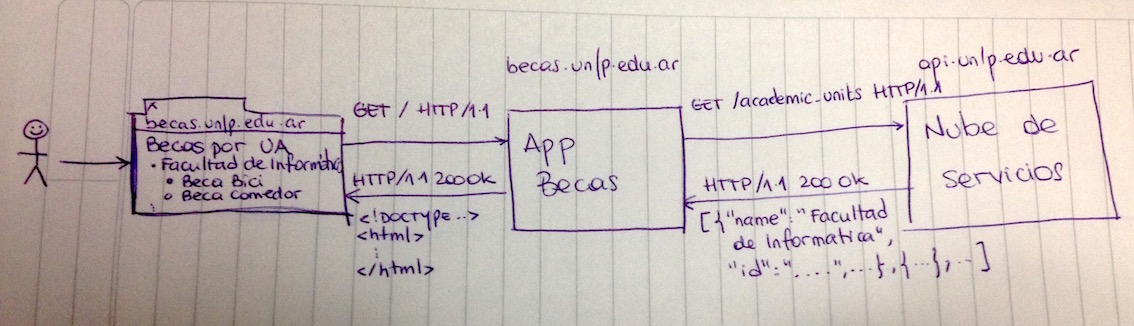
\includegraphics[width=\linewidth]{src/images/01-capitulo-1/ejemplo-rest-becas.jpg}
  \caption{Interacciones involucradas.}
  \label{fig:ejemplo-rest-becas}
\end{figure}

En la sección \ref{standard:rest} realizaremos el desarrollo pertinente de la definición de la arquitectura de aplicaciones distribuidas \gls{acro:rest} que Fielding publicó, dando de esa forma un marco teórico adecuado a las definiciones de nuestra nueva arquitectura para la nube de servicios.


\paragraph{El diseño final: el Integrador}

Luego de analizar las posibilidades que brindaba el uso de los principios \gls{acro:rest} en detalle, realizamos el primer diseño de cómo quedarían definidos los distintos servicios o \gls{term:endpoint} y decidimos darle un nombre: el \textit{Integrador}, una mezcla entre título de historieta\footnote{En cierto modo, nos recuerda historietas como Castigador (\eng{The Punisher}, de \eng{Marvel Comics}) – https://es.wikipedia.org/wiki/Punisher} y \eng{Terminator}, que nos acompaña hasta el día de hoy cuando hacemos referencia a la aplicación \textit{detrás} de la nube de servicios.

Realizando un enfoque más pragmático que correcto para el diseño, definimos servicios que retornan documentos \gls{lang:json} para cada una de las entidades que se podían consultar sin realmente analizar si serían realmente útiles, o si siquiera se accederían alguna vez. Fue de esta forma que la \gls{acro:api} se compuso de los más de 100 \gls{term:endpoint} que tiene hoy, que no siguen una misma línea en su diseño,  no tienen una estructura estándar de respuesta, y de los cuales efectivamente se usa tan solo el 46\%\footnote{Esta cifra surge de los datos que tenemos en nuestra herramienta de analíticas. De los 105 servicios que existen, 56 no registran accesos en el último año.}. A continuación listamos todos los servicios provistos por la nube, identificados por los patrones de sus URLs (omitiremos el dominio y el protocolo para simplificar la lista):

% TODO: Acomodar esto y limpiarlo un poco, es una negrada. Al menos llevarlo a un anexo.
\begingroup
  \begin{itemize}
    \item \lstinline$/api/academic_data.json/:id$
    \item \lstinline$/api/academic_degree_type.json$
    \item \lstinline$/api/academic_degree_type.json/:id$
    \item \lstinline$/api/academic_degree_type.json/count$
    \item \lstinline$/api/academic_unit.json$
    \item \lstinline$/api/academic_unit.json/:id$
    \item \lstinline$/api/academic_unit.json/count$
    \item \lstinline$/api/academic_unit/:id/academic_unit_college_degree.json$
    \item \lstinline$/api/academic_unit/:id/academic_unit_college_degree.json/count$
    \item \lstinline$/api/academic_unit/:id/career.json$
    \item \lstinline$/api/academic_unit/:id/career.json/count$
    \item \lstinline$/api/academic_unit/:id/career/:career_id/career_programme.json$
    \item \lstinline$/api/academic_unit/:id/career/:career_id/career_programme.json/count$
    \item \lstinline$/api/academic_unit/:id/career/:career_id/career_programme/:career_programme_id/career_programme_degree.json$
    \item \lstinline$/api/academic_unit/:id/career/:career_id/career_programme/:career_programme_id/career_programme_degree.json/count$
    \item \lstinline$/api/academic_unit/:id/career/:career_id/career_programme/:career_programme_id/career_subject.json$
    \item \lstinline$/api/academic_unit/:id/career/:career_id/career_programme/:career_programme_id/career_subject.json/count$
    \item \lstinline$/api/academic_unit/:id/degree.json$
    \item \lstinline$/api/academic_unit/:id/degree.json/count$
    \item \lstinline$/api/academic_unit/:id/degree/:degree_id/career_programme_degree.json$
    \item \lstinline$/api/academic_unit/:id/degree/:degree_id/career_programme_degree.json/count$
    \item \lstinline$/api/academic_unit/:id/paycheck.json$
    \item \lstinline$/api/academic_unit/:id/paycheck.json/count$
    \item \lstinline$/api/academic_unit/:id/paycheck.json/search/:query$
    \item \lstinline$/api/academic_unit/:id/paycheck.json/search/:query/count$
    \item \lstinline$/api/academic_unit/:id/person.json$
    \item \lstinline$/api/academic_unit/:id/person.json/count$
    \item \lstinline$/api/academic_unit/:id/person.json/search/:query$
    \item \lstinline$/api/academic_unit/:id/person.json/search/:query/count$
    \item \lstinline$/api/academic_unit_college_degree.json/:id$
    \item \lstinline$/api/career.json/:id$
    \item \lstinline$/api/career_programme.json/:id$
    \item \lstinline$/api/career_programme_degree.json/:id$
    \item \lstinline$/api/career_subject.json/:id$
    \item \lstinline$/api/census_data.json/:id$
    \item \lstinline$/api/city.json/:id$
    \item \lstinline$/api/country.json$
    \item \lstinline$/api/country.json/:id$
    \item \lstinline$/api/country.json/count$
    \item \lstinline$/api/country/:id/state.json$
    \item \lstinline$/api/country/:id/state.json/count$
    \item \lstinline$/api/country/:id/state/:state_id/department.json$
    \item \lstinline$/api/country/:id/state/:state_id/department.json/count$
    \item \lstinline$/api/country/:id/state/:state_id/department/:department_id/city.json$
    \item \lstinline$/api/country/:id/state/:state_id/department/:department_id/city.json/count$
    \item \lstinline$/api/degree.json/:id$
    \item \lstinline$/api/department.json/:id$
    \item \lstinline$/api/document_type.json$
    \item \lstinline$/api/document_type.json/:id$
    \item \lstinline$/api/document_type.json/count$
    \item \lstinline$/api/gender.json$
    \item \lstinline$/api/gender.json/:id$
    \item \lstinline$/api/gender.json/count$
    \item \lstinline$/api/marital_status.json$
    \item \lstinline$/api/marital_status.json/:id$
    \item \lstinline$/api/marital_status.json/count$
    \item \lstinline$/api/official_scale.json$
    \item \lstinline$/api/official_scale.json/:id$
    \item \lstinline$/api/official_scale.json/count$
    \item \lstinline$/api/official_scale/:id/personal_scale.json$
    \item \lstinline$/api/official_scale/:id/personal_scale.json/count$
    \item \lstinline$/api/paycheck.json/:id$
    \item \lstinline$/api/person.json$
    \item \lstinline$/api/person.json/:id$
    \item \lstinline$/api/person.json/count$
    \item \lstinline$/api/person.json/search/:id$
    \item \lstinline$/api/person/:id/academic_data.json$
    \item \lstinline$/api/person/:id/academic_data.json/count$
    \item \lstinline$/api/person/:id/academic_unit/:academic_unit_id/paycheck.json$
    \item \lstinline$/api/person/:id/academic_unit/:academic_unit_id/paycheck.json/count$
    \item \lstinline$/api/person/:id/academic_unit/:academic_unit_id/paycheck.json/search/:query$
    \item \lstinline$/api/person/:id/academic_unit/:academic_unit_id/paycheck.json/search/:query/count$
    \item \lstinline$/api/person/:id/census_data.json$
    \item \lstinline$/api/person/:id/census_data.json/count$
    \item \lstinline$/api/person/:id/is_graduated.json/:query_1/:query_2/:query_3$
    \item \lstinline$/api/person/:id/paycheck.json$
    \item \lstinline$/api/person/:id/paycheck.json/count$
    \item \lstinline$/api/person/:id/paycheck.json/search/:query$
    \item \lstinline$/api/person/:id/paycheck.json/search/:query/count$
    \item \lstinline$/api/person/:id/person_email.json$
    \item \lstinline$/api/person/:id/person_email.json/count$
    \item \lstinline$/api/person/:id/person_high_study.json$
    \item \lstinline$/api/person/:id/person_high_study.json/count$
    \item \lstinline$/api/person/:id/person_role.json$
    \item \lstinline$/api/person/:id/person_role.json/count$
    \item \lstinline$/api/person/:id/personal_age.json$
    \item \lstinline$/api/person/:id/personal_age.json/count$
    \item \lstinline$/api/person/:id/personal_charge.json$
    \item \lstinline$/api/person/:id/personal_charge.json/count$
    \item \lstinline$/api/person_email.json/:id$
    \item \lstinline$/api/person_high_study.json/:id$
    \item \lstinline$/api/person_role.json/:id$
    \item \lstinline$/api/personal_age.json/:id$
    \item \lstinline$/api/personal_charge.json/:id$
    \item \lstinline$/api/personal_scale.json/:id$
    \item \lstinline$/api/state.json/:id$
    \item \lstinline$/api/student_status.json$
    \item \lstinline$/api/student_status.json/:id$
    \item \lstinline$/api/student_status.json/count$
    \item \lstinline$/api/study_category.json$
    \item \lstinline$/api/study_category.json/:id$
    \item \lstinline$/api/study_category.json/count$
    \item \lstinline$/api/study_category/:id/study_type.json$
    \item \lstinline$/api/study_category/:id/study_type.json/count$
    \item \lstinline$/api/study_type.json/:id$
  \end{itemize}
\endgroup


Sin entrar en detalles sobre cada punto, se puede observar claramente la falta de consistencia en la definición de las \glspl{acro:url}, la sobrecarga de niveles de anidamiento en servicios como el que devuelve las materias del plan de estudios de una carrera de una Unidad Académica (\lstinline$/api/academic_unit/:id/career/:career_id/career_programme/:career_programme_id/career_subject.json$) que anida esos 3 niveles para mostrar la información, aunque los identificadores únicos de cada elemento podrían usarse, en una estructura más plana, para acceder directamente al último nivel, algo así como (\lstinline$/api/career_programme/:career_programme_id/career_subject.json$) y así simplificar las \glspl{acro:url}.

Estos problemas sumados a la falta de documentación sobre cómo usar los diferentes servicios, qué parámetros reciben y qué estructura tiene la respuesta cada uno, hacen más complejo el uso de esta \gls{acro:api} tanto para desarrolladores que la venimos utilizando hace tiempo, como para nuevos integrantes del equipo a los que queremos sumar a alguna aplicación que haga uso de estos servicios.

\paragraph{El Integrador: implementación}

La nube de servicios, como aplicación, fue un desarrollo más realizado en PHP 5 y el framework \gls{fw:symfony} 1.4, utilizando MySQL como motor para las 5 bases de datos que utiliza para proveer la información:

\begin{itemize}
  \item Una base de datos donde se almacena información propia de la aplicación: tokens de acceso, estadísticas de acceso, información de clientes de la \gls{acro:api}.
  \item Una segunda base de datos para los datos de referencia de los que ya hemos hablado (tipos de documento, países, etcétera).
  \item Una tercera base en la que se mantiene actualizada la información que nos llega desde la oficina de Liquidaciones del CeSPI, la cual se transforma mediante procesos \gls{acro:etl}\footnote{Técnica que se utiliza para tomar datos de una o múltiples fuentes de información, modificarla y cargarla en una o más almacenes de datos. En nuestro caso utilizamos la herramienta Kettle de la versión de comunidad de la suite Pentaho para transformar los datos fuente, que nos llegan en archivos de texto plano, en inserciones normalizadas en nuestra base de datos MySQL.}\cite{paper:etl} para normalizarla antes de guardarla en esta base de datos.
  \item Una cuarta para la información que proviene de los SIU Guarani de las distintas Unidades Académicas, la cual es actualizada directamente por el grupo de Sistemas Académicos del \cespi.
  \item Y una quinta base de datos donde se unifican y mezclan los datos de las últimas 3 bases datos mencionadas, de manera tal que se logre una trazabilidad de la persona como un todo a lo largo de su \textit{vida en la UNLP}, ya sea como alumno, docente o nodocente.
\end{itemize}

La aplicación se realizó sin considerar algunos aspectos claves para mejorar la \eng{performance} del lado de los clientes de la \gls{acro:api}, como puede ser utilizar cabeceras de \eng{caching}, compresión de respuestas, utilizar \eng{caches} compartidas y otras estrategias que desarrollaremos más en detalle como parte de nuestro análisis para el futuro de la nube de servicios.

Para las \gls{term:aplicacionessatelitales}, se realizó un \eng{plugin} de \gls{fw:symfony} que abstraía en clases y objetos la mayoría de los servicios existentes, implementando cierto mecanismo de caching local a cada aplicación, pero que al ser decisiones realizadas meramente del lado del cliente, existían situaciones en las que la información almacenada en esa cache local quedaba \eng{stale} (desactualizada) con respecto a lo que la \gls{acro:api} devolvía como el dato \eng{fresh}, por lo que se debió implementar en algunos casos un mecanismo manual de vaciado de \eng{cache} para subsanar estas situaciones.

En resumen: la implementación fue adecuada y funcional para las necesidades del momento, pero con el tiempo esas necesidades y, principalmente, la tecnología fueron cambiando, lo cual fue acrecentando gradualmente la necesidad de un nuevo análisis y replanteo para la solución actual.


\subsubsection{Cuarta iteración: este trabajo}
\label{nube:etapa4}

Mucha agua ha pasado bajo el puente desde que implementamos la versión actual de la nube de servicios de la UNLP, y varios han sido los cambios que el paso de estos 4 años nos ha dejado: pasamos de ser un equipo de alrededor de 8 personas en que todos nos dedicábamos a desarrollar aplicaciones web en PHP con el framework \gls{fw:symfony}, algunos toques de JavaScript para la interfaz de usuario y bases de datos MySQL, a ser un equipo de 17 personas que desarrolla aplicaciones en el lenguaje Ruby, con \gls{fw:rails} y \gls{fw:sinatra} como \eng{frameworks} web de cabecera, realizando algunas pequeñas aplicaciones meramente en JavaScript, que ha reescrito en Ruby varias de las aplicaciones realizadas en PHP y mantiene activamente aquellas desarrolladas en \gls{fw:symfony} que aún no se han migrado, utilizando bases de datos MySQL mayoritariamente y en algunos casos combinándolas con bases de datos \gls{db:nosql} y almacenes clave-valor en memoria, como \gls{db:redis} o \gls{db:memcached}. Estos cambios han traído aparejada la implementación de un cliente desarrollado en Ruby para integrarlo, de la misma forma que lo hicimos en el caso de las aplicaciones PHP, en las aplicaciones basadas en \gls{fw:rails} y \gls{fw:sinatra}. Este fue otro caso más donde las limitaciones del Integrador actual debieron ser sorteadas mediante la adición de lógica del lado del cliente:

\begin{itemize}
  \item Las aplicaciones cliente desarrolladas en Ruby implementan una cache condicional basada en \gls{db:redis} o en archivos del filesystem (según disponibilidad, y en ese orden de prioridad), que almacena las respuestas a los requerimientos por un tiempo determinado\footnote{La posibilidad de especificar el tiempo por el cual se desea guardar la copia en cache (el \gls{acro:ttl}) fue agregada recién en Abril de 2015, es decir que antes se almacenaban indefinidamente las copias en \eng{cache}, lo que para los casos en que se usaba el sistema de archivos como almacenamiento esto representaba un potencial problema de crecimiento sin tope de los archivos utilizados para la cache.} e intenta subsanar la falta de directivas de cabeceras de parte de la \gls{acro:api} de servicios.

  \item Al no tener un estándar para la estructura de las respuestas, la lógica de hidratación de éstos documentos \gls{lang:json} para convertirlos en objetos del dominio de las aplicaciones es excesivamente costosa en términos de \eng{performance} y tiene varios chequeos que podrían evitarse si se normalizaran y estandarizasen las respuestas.

  \item La falta de documentación nos ha obligado en ocasiones teniendo que hacer una suerte de ingeniería inversa de las respuestas para entender relaciones entre datos.
\end{itemize}

Otro gran problema es la dificultad para escalar que tiene la arquitectura actual. La aplicación web que atiende los pedidos a la nube y sus 5 bases de datos viven en una misma máquina virtual, lo cual puede ser hasta cierto punto conveniente para tener un mantenimiento y administración centralizados, pero esto acota en gran medida la posibilidad de poner rápidamente en funcionamiento nuevas instancias de la \gls{acro:api} que puedan balancear proporcionalmente la carga ante la creciente demanda que tiene por parte de las aplicaciones cliente. Este único punto de falla también es un potencial riesgo en caso de intrusiones o caídas de cualquier índole: fallas eléctricas, de red, de disco o errores humanos a la hora de realizar el mantenimiento de ese equipo virtual. Las tecnologías que utiliza ya no son mantenidas por sus desarrolladores: PHP 5.3 alcanzó su \eng{end of life} el 14 de Agosto de 2014\footnote{Cf. http://php.net/eol.php} y \gls{fw:symfony} 1.4 dejó de ser mantenido en Noviembre de 2012\footnote{Cf. http://symfony.com/blog/symfony-1-4-end-of-maintenance-what-does-it-mean}, lo cual implica que en cierto modo la aplicación puede eventualmente ser víctima de nuevas vulnerabilidades que se descubran a esa rama del desarrollo y que ya no serán solucionadas.

Todos estos cambios y problemas motivan el presente trabajo, en el cual analizaremos las posibilidades que ofrece una \gls{acro:api} diseñada desde el comienzo con el nivel más alto\footnote{Así define Leonard Richardson el conjunto de requerimientos para alcanzar un servicio que cumpla realmente con todos los principios que Roy Fielding definió para una \gls{acro:api} \gls{acro:rest}, y define que \gls{acro:hateoas} es el requerimiento de nivel 3 para alcanzar la pureza de \gls{acro:rest}. – http://www.crummy.com/writing/speaking/2008-QCon/act3.html y claramente analizado por Martin Fowler en http://martinfowler.com/articles/richardsonMaturityModel.html} de adhesión a \gls{acro:rest} posible (\gls{term:hypermedia}), basándonos en estándares ya establecidos en lugar de intentar reinventar la rueda y definir el nuestro propio para las respuestas \gls{lang:json}, pensando en aprovechar las posibilidades de caching que ofrecen las distintas capas del diseño, e intentando descentralizar la información de manera tal que se elimine el único punto de falla que existe en la actualidad y que nos permita escalar horizontalmente en cantidad de instancias de la nube de manera transparente y poco costosa.
